\chapter{Neutrino physics} %%%%%%%%%%%%%%%%%%%%%%%%%%%%%%%%%%%%%%%%%%%%%%%%%%%%%%%%%%%%%%%%%%%%%%%
\label{chap:theory} %%%%%%%%%%%%%%%%%%%%%%%%%%%%%%%%%%%%%%%%%%%%%%%%%%%%%%%%%%%%%%%%%%%%%%%%%%%%%%

Vast numbers of neutrinos pass through everything that surrounds us each second, each one
incredibly unlikely to interact even once. Nearly a century since they were first proposed, these
mysterious particles have now conclusively been proven to undergo oscillations between their
flavour states. This profound discovery has opened the door to physics beyond that initially
conceived within the Standard Model, which may reveal new, fundamental insights into the universe.
This chapter aims to outline the historical context, theoretical background and open questions
surrounding the neutrino.

\section{A history} %%%%%%%%%%%%%%%%%%%%%%%%%%%%%%%%%%%%%%%%%%%%%%%%%%%%%%%%%%%%%%%%%%%%%%%%%%%%%%
\label{sec:theory_history} %%%%%%%%%%%%%%%%%%%%%%%%%%%%%%%%%%%%%%%%%%%%%%%%%%%%%%%%%%%%%%%%%%%%%%%

\subsection{Discovery of the neutrinos} %%%%%%%%%%%%%%%%%%%%%%%%%%%%%%%%%%%%%%%%%%%%%%%%%%%%%%%%%%
\label{sec:theory_history_neutrinos} %%%%%%%%%%%%%%%%%%%%%%%%%%%%%%%%%%%%%%%%%%%%%%%%%%%%%%%%%%%%%

In the early 20th century, beta decays were assumed to follow the simple two-body process,
$A\rightarrow B + e$, where $A$ spontaneously emits a single electron. To conserve both energy and
angular momentum, the ejected electron was believed to have discrete kinetic energy defined by the
difference in binding energies between $A$ and $B$. However, in 1914, J. Chadwick instead measured
a continuous electron energy spectrum~\cite{chadwick1914}, placing this assumption in doubt.

W. Pauli proposed a `desperate solution' to this paradox in 1930~\cite{pauli1930}. If a light,
neutrally charged, spin $1/2$ particle was also produced in the interaction, the continuous energy
distribution could be explained. Initially, this peculiar new particle was named the
\emph{neutron}. However, to avoid confusion with the heavy baryon of the same name discovered in
1932, E. Fermi renamed it the \emph{neutrino} when he formalised his theory of beta decay in
1934~\cite{fermi1934}.

The same year, H. Bethe and R. Peierls~\cite{bethe1934} used Fermi's work to estimate the
cross-section for the inverse beta decay process
\begin{equation} % INVERSE BETA DECAY EQUATION %
    \bar{\nu} + p^{+} \rightarrow n + e^{+}.
    \label{eq:inverse_beta_decay}
\end{equation}
They calculated an upper limit of $\sigma<10^{-44} \text{cm}^2$ for neutrinos of energy
\unit{2.3}{\MeV}, an incredibly small value. When summarising, they declared that `it seems highly
improbable that, even for cosmic ray energies, $\sigma$ becomes large enough to allow the process
to be observed'. Although this estimation did not prove accurate and extensive neutrino
observations have since been made, it hinted at the great difficulties experimentalists would face
measuring the neutrino in the years to come.

After an initial tentative identification in 1953, F. Reines and C. Cowan made the first confirmed
observation of the neutrino in 1956~\cite{cowan1956}. Electron antineutrinos produced within the
Savannah River Plant nuclear reactor were detected via the inverse beta decay process outlined in
Eq.~\ref{eq:inverse_beta_decay}. In an underground room of the reactor building, a `club-sandwich'
detector was constructed containing three \unit{1500}{\text{litre}} liquid scintillator tanks
interspersed with two \unit{200}{\text{litre}} cadmium doped water target tanks. A total of 330
photomultiplier tubes then measured the characteristic signal for the interaction, a positron
annihilation followed shortly afterwards by a gamma-ray burst from the neutron capture.

A second distinct neutrino, the muon neutrino, was discovered in 1962 at the Brookhaven based
Alternating Gradient Synchrotron (AGS)~\cite{danby1962}. Protons from the AGS beam incident upon a
fixed target produced charged pions which then decayed into a beam of muons and neutrinos. After
passing through steel and lead absorbers to remove the muons, neutrino interactions were detected
in a series of downstream spark chambers.

If only a single neutrino existed, both interactions
\begin{equation} % BROOKHAVEN DECAY EQUATIONS %
    \nu+p^{+}\rightarrow\mu^{+}+n, \\
    \nu+p^{+}\rightarrow e^{+}+n,
\end{equation}
were expected to occur at the same rate. However, only muons, identified by a single long track in
the spark chambers, were detected, confirming the existence of the muon neutrino. Not only was
this experiment the first to construct and use an artificial neutrino beam, but it also won the
1988 Nobel Prize in Physics.

The $Z^{0}$ and $W^{\pm}$ bosons were discovered at the CERN based Super Proton Synchrotron in
1983~\cite{arnison1983_z, arnison1983_w}. Crucially, as $Z^{0}$ bosons were expected to decay to
neutrinos, measurements made to the decay width could strongly constrain the number of neutrino
flavours. The ALEPH, DELPHI, L3, and OPAL experiments at the LEP $e^{+}e^{-}$ collider in the
1990s made such precise measurements (see Fig.~\ref{fig:z_resonance}), indicating that the number
of light active neutrino flavours was $2.984\pm0.008$~\cite{electroweak2006}.

\begin{figure} % Z-RESONANCE DIAGRAM %
    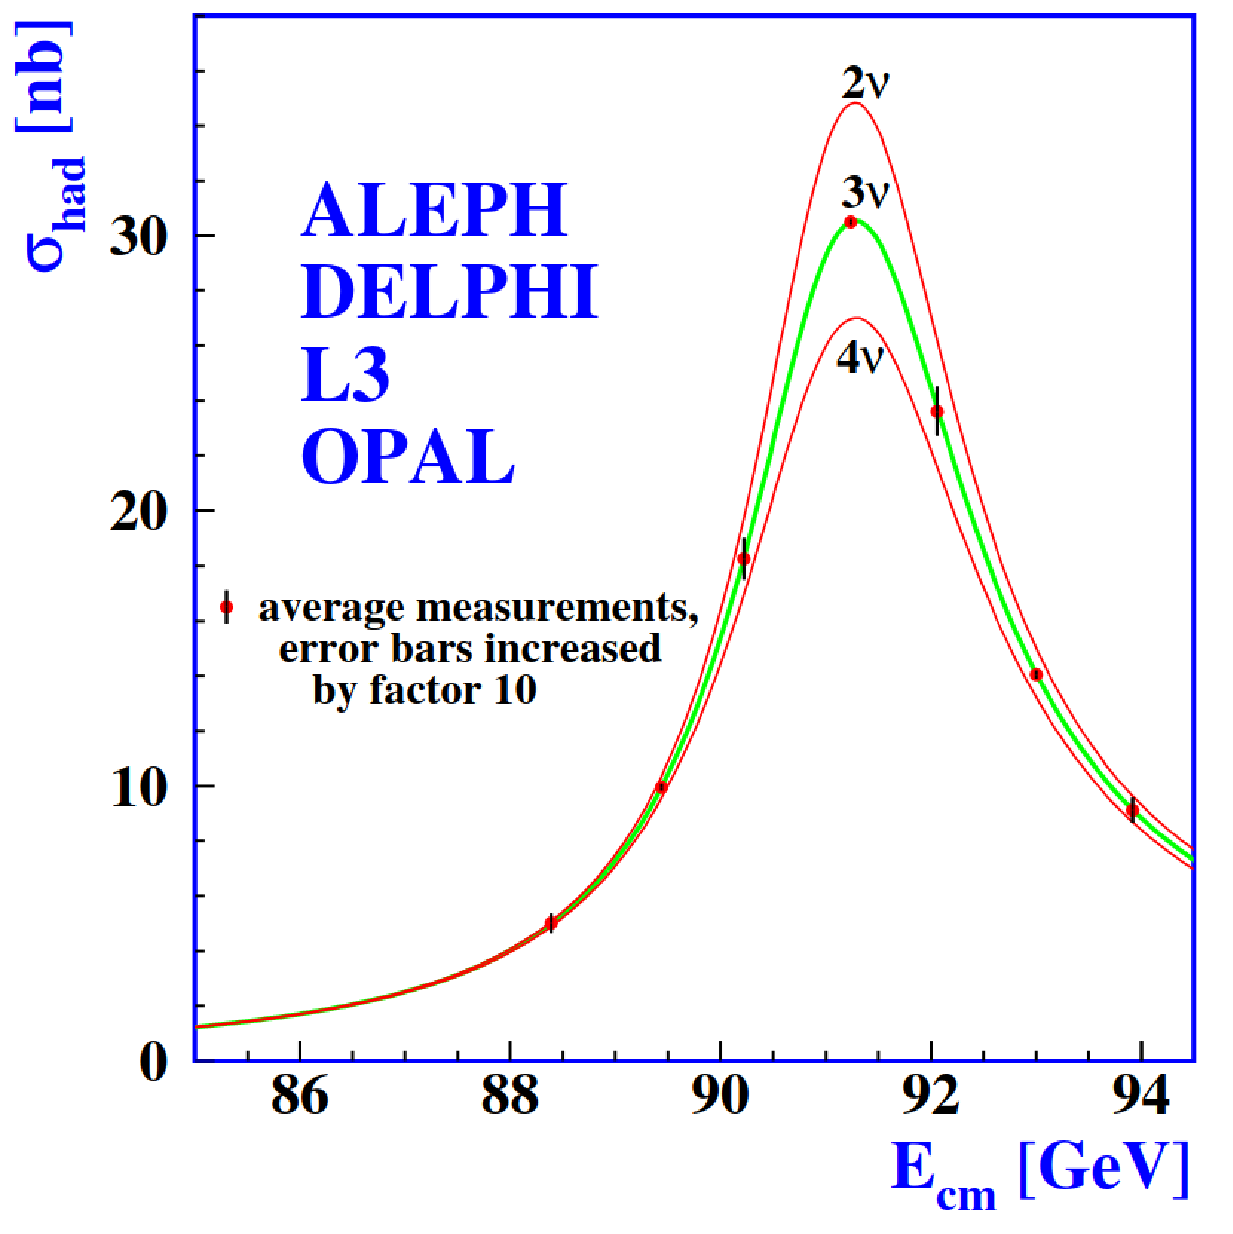
\includegraphics[origin=c,width=0.5\textwidth]{diagrams/3-theory/z_resonance.pdf}
    \caption[Hadron production cross-section measurements from LEP]
    {Combined hadron production cross-section measurements around the $Z^{0}$ resonance made by
        the LEP experiments. The curves show the predicted cross-section for two, three, and four
        neutrinos. Note how the data fits the three active neutrino hypothesis incredibly well.
        Figure taken from Ref.~\cite{electroweak2006}.}
    \label{fig:z_resonance}
\end{figure}

This indication from LEP combined with the discovery of the charged tau lepton in
1975~\cite{perl1975} made the existence of a third tau neutrino extremely likely. The Fermilab
based DONUT experiment finally discovered this particle in 2001 using \unit{800}{\GeV} protons
from the Tevatron~\cite{Kodama2001}, completing the trio of active neutrinos we know today.
However, additional \emph{sterile} neutrino flavours which do not couple to the weak force are
still a possibility, with various hints to their existence having been
observed~\cite{particle2020}.

\subsection{Discovery of neutrino oscillations} %%%%%%%%%%%%%%%%%%%%%%%%%%%%%%%%%%%%%%%%%%%%%%%%%%
\label{sec:theory_history_osc} %%%%%%%%%%%%%%%%%%%%%%%%%%%%%%%%%%%%%%%%%%%%%%%%%%%%%%%%%%%%%%%%%%%

At the Homestake mine in the 1960s, a \unit{400000}{\text{litre}} tank, placed
\unit{1.5}{\text{km}} underground, was filled with the dry cleaning fluid perchloroethylene
($C_{4}Cl_{8}$). Its goal was to measure the electron neutrino flux incident upon the Earth from
the Sun via the interaction
\begin{equation} % HOMESTAKE CHLORINE EQUATION %
    {}^{37}Cl+\nu_{e}\rightarrow{}^{37}Ar+e^{-}.
    \label{eq:homestake}
\end{equation} %
This process (Eq.~\ref{eq:homestake}) allowed the neutrino flux to convert the chlorine contained
within the tank into the noble gas argon. Every few weeks the tank was purged with gaseous helium
and the amount of argon generated, and indirectly the solar neutrino flux measured.

After analysis, the number of electron neutrino interactions per ${}^{37}Cl$ per second, was found
to be no greater than 3~\cite{davis1968}. When compared to the predictions made by the Standard
Solar Model ranging between 4.4 and 22~\cite{bahcall1968}, a deficit was observed. Dubbed the
\emph{solar neutrino problem}, this was initially believed to be due to an unexplained
experimental flaw. However, other experiments, such as the water Cherenkov Kamiokande
II~\cite{hirata1989} and the SAGE and GALLEX galium based capture tanks also observed this
discrepancy~\cite{abazov1991, anselmann1994}.

A second deficit, the \emph{atmospheric neutrino anomaly}, was also indirectly observed for
neutrinos generated in the Earth's upper atmosphere by cosmic rays. Such neutrinos formed a key
background to both the Kamiokande and IMD experiments, which were primarily designed to measure
proton decay. When evaluating their backgrounds, a deficit in the number of muon neutrinos
compared to electron neutrinos was observed~\cite{hirata1988, becker1992}. The successor to the
Kamiokande experiment, Super-Kamiokande also measured a similar deficit~\cite{kajita1999}.

The phenomenon of neutrino oscillations was put forward as a solution to this problem. If
neutrinos could change flavour as they propagated, the measured deficits could be explained. The
SNO experiment finally confirmed such oscillations in 2001~\cite{ahmad2002}.

SNO consisted of a \unit{1}{\text{kton}} tank of deuterium (heavy water), equipped with 9500
photomultiplier tubes. Light from three separate neutrino interaction channels:
\begin{align} % SNO INTERACTIONS EQUATIONS %
    \nu_{i}+e^{-} & \rightarrow \nu_{i}+e^{-}, \\
    \nu_{i}+d     & \rightarrow p+n+\nu_{i},   \\
    \nu_{e}+d     & \rightarrow p+p+e^{-},
\end{align}
was measured, where $d$ is the deuterium nucleus. The first and second channels were sensitive to
all three neutrino flavours, but crucially only electron neutrinos could interact via the third
channel. By comparing the relative rates between the channels, SNO was able to prove to
5.3$~\sigma$ that electron neutrinos had oscillated to other flavours.

\section{The Standard Model and neutrinos} %%%%%%%%%%%%%%%%%%%%%%%%%%%%%%%%%%%%%%%%%%%%%%%%%%%%%%%
\label{sec:theory_sm} %%%%%%%%%%%%%%%%%%%%%%%%%%%%%%%%%%%%%%%%%%%%%%%%%%%%%%%%%%%%%%%%%%%%%%%%%%%%

The Standard Model of particle physics describes the seventeen known fundamental subatomic
particles and their interactions. Combining both quantum chromodynamics (describing the strong
force) and electroweak theory (describing the electromagnetic and weak forces), the Standard Model
is a gauge theory obeying the local gauge symmetries of $U(1) \times SU(2) \times SU(3)$. The
particles, along with their various properties, are outlined in Fig.~\ref{fig:sm}. Additionally,
all have an associated anti-particle with the same quantum numbers except the electric charge,
which is opposite.

\begin{figure} % STANDARD MODEL DIAGRAM %
    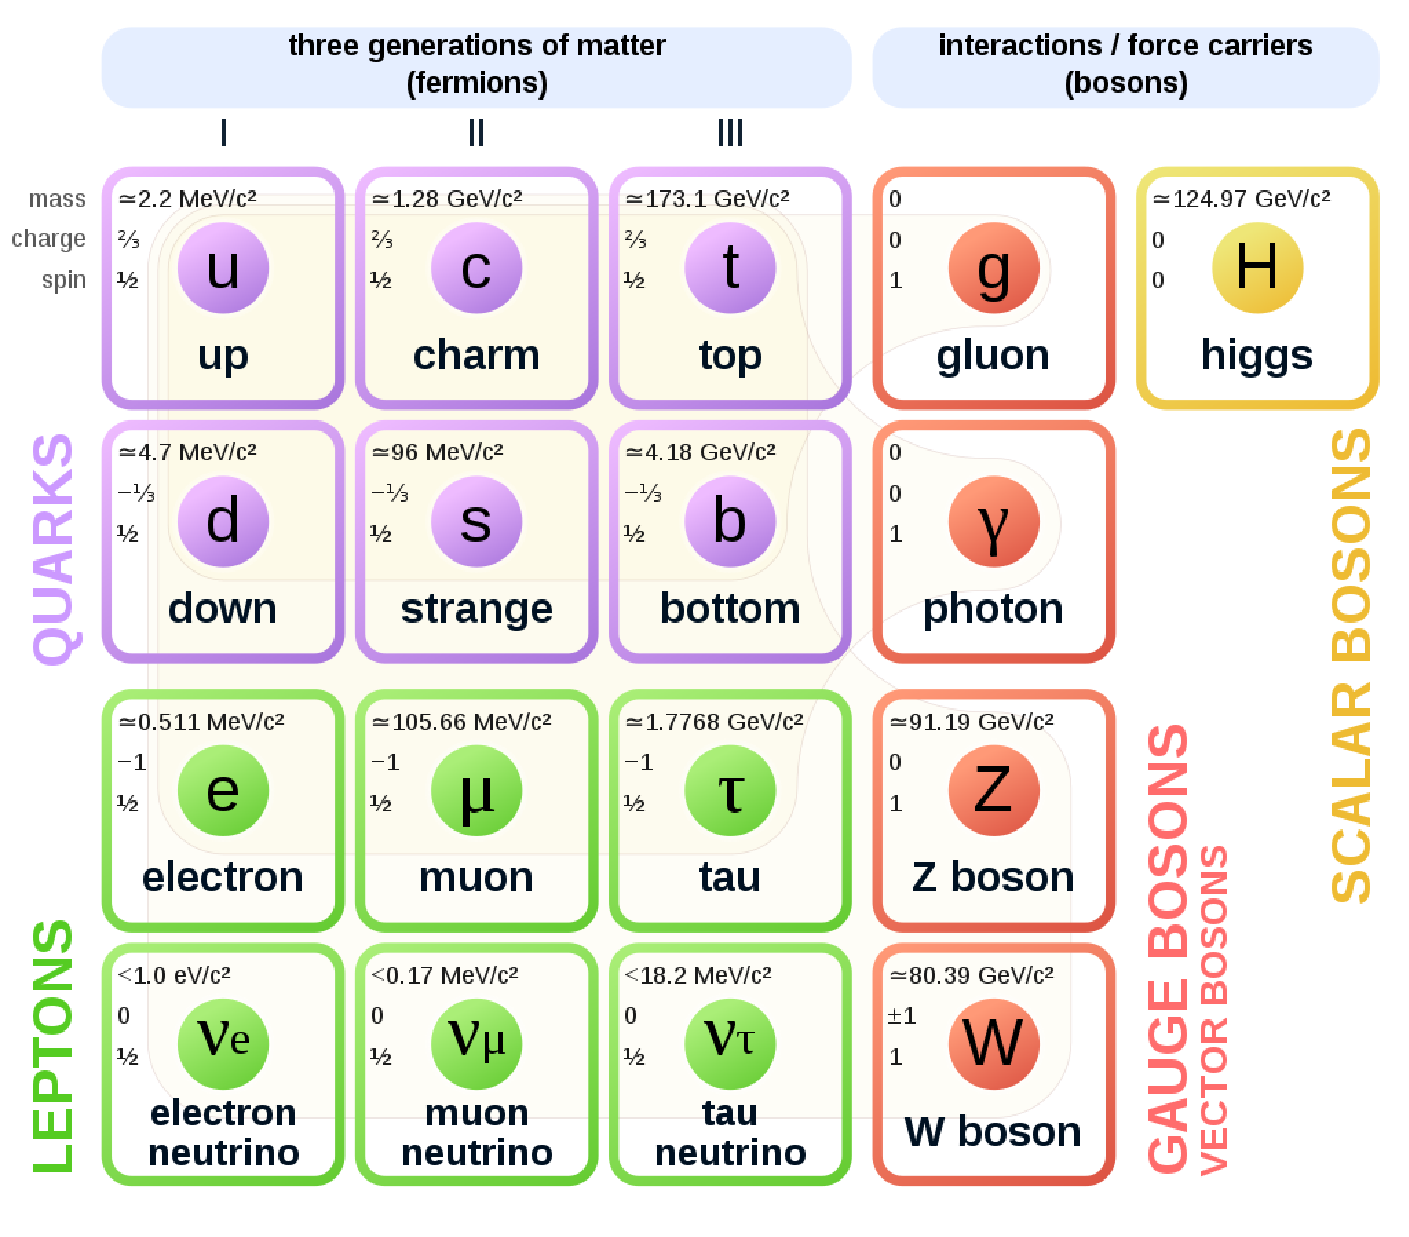
\includegraphics[origin=c,width=0.5\textwidth]{diagrams/3-theory/sm.pdf}
    \caption[The particles of the Standard Model]
    {The particles of the Standard Model, including the quarks, leptons, and bosons. Figure taken
        from Ref.~\cite{wiki2020}.}
    \label{fig:sm}
\end{figure}

The six quarks and six leptons, all spin $1/2$ particles, are named fermions. Further divided into
three generations (or flavours), they make up all the matter content of the universe. The quarks
never exist in a free state and bind together into mesons or baryons, such as pions and protons,
respectively.  Three charged massive particles, the electron, the muon, and the tau and their
three corresponding (initially assumed to be massless) neutrinos, make up the leptons.

The spin 1 gauge bosons carry the electromagnetic, strong, and weak forces. The photon carries the
electromagnetic force (affecting all charged particles), the gluons carry the strong force (which
binds the quarks together), and the massive $Z^{0}$ and $W^{\pm}$ carry the weak force. The final
particle, the Higgs, is a massive scalar boson. Via the process of spontaneous symmetry breaking,
the Higgs provides the mechanism to give the particles their mass.

Within the Standard Model, neutrinos only interact via the weak force, exclusively coupling to the
$Z^{0}$ and $W^{\pm}$ bosons. As the weak interaction maximally violates parity, in that it only
couples to left-handed chiral particles, the original Standard Model only contains left-handed
neutrinos and their corresponding right-handed anti-neutrinos.

Although neutrinos were initially thought to be massless, and no direct detection of their mass
has been made, it is now believed that neutrinos are massive (albeit very light) particles. This
belief is due to the substantial amount of evidence in support of neutrino oscillations, such as
the result from SNO amongst others detailed in Section.~\ref{sec:theory_status}. These
oscillations require three distinct neutrino mass states, implying at least two are non-zero.

The Standard Model does not strictly rule out massive neutrinos which are permitted as either
\emph{Dirac} or \emph{Majorana} particles. If neutrinos are Dirac in nature, they acquire their
mass via a Yukawa coupling, just like the other fermions. This coupling mixes both left-handed and
right-handed fields, requiring the existence of right-handed neutrinos (left-handed antineutrinos)
that do not interact via the weak force. Conversely, if neutrinos are Majorana in nature, a mass
term can be introduced containing just the left-handed neutrino states. This term requires that
the neutrino is its own anti-particle, which as neutrinos do not carry a charge, is
possible~\cite{particle2020}.

Strongly model-dependent cosmological observations of the cosmic microwave background currently
provide the best limit on the combined sum of the neutrino masses at $\sum m_{\nu} <
    0.12~\eV$~\cite{planck2018}. Furthermore, the KATRIN experiment has been able to make
model-independent direct measurements of the upper mass limit by looking at the energy spectrum of
electrons emitted from beta decay, giving a result of $m_{\nu} < 1.1~\eV$~\cite{aker2019}.

\section{Neutrino oscillations} %%%%%%%%%%%%%%%%%%%%%%%%%%%%%%%%%%%%%%%%%%%%%%%%%%%%%%%%%%%%%%%%%%
\label{sec:theory_oscillations} %%%%%%%%%%%%%%%%%%%%%%%%%%%%%%%%%%%%%%%%%%%%%%%%%%%%%%%%%%%%%%%%%%

B. Pontecorvo, Z. Maki, M. Nakagawa, and S. Sakata developed the theory of neutrino oscillations
in the 1960s~\cite{maki1962, pontecorvo1967, pontecorvo1969}. Fundamentally, it is a manifestation
of the phenomenon of quantum interference. If neutrinos are massive, their mass eigenstates are
not necessarily the same as their weakly interacting flavour eigenstates. Instead, the flavour
states are a superposition of the three mass states, each propagating as distinct waves evolving
differently with time. As a direct consequence of this, if a neutrino is created with a specific
flavour $\alpha$, its flavour composition will change with time, such that it may later be
detected as having a flavour $\beta$. The probability of this change is found to be periodic
(hence oscillations) and dependent on the neutrino energy, the propagation distance, and a
rotational mixing matrix.

\subsection{Neutrino mixing} %%%%%%%%%%%%%%%%%%%%%%%%%%%%%%%%%%%%%%%%%%%%%%%%%%%%%%%%%%%%%%%%%%%%%
\label{sec:theory_oscillations_mixing} %%%%%%%%%%%%%%%%%%%%%%%%%%%%%%%%%%%%%%%%%%%%%%%%%%%%%%%%%%%

The mixing between the flavour eigenstates $\ket{\nu_{\alpha}}$, where $\alpha=e,\mu,\tau$, and
the mass eigenstates $\ket{\nu_{k}}$, where $k=1,2,3$, is described by the
\emph{Pontecorvo-Maki-Nakagawa-Sakata} (PMNS) matrix $U$, such that
\begin{equation} % FLAVOUR AS MASS EQUATION %
    \ket{\nu_{\alpha}}=\sum_{k}^{3}U_{\alpha k}^{*}\ket{\nu_{k}},
\end{equation}
and vice-versa,
\begin{equation} % MASS AS FLAVOUR EQUATION %
    \ket{\nu_{k}}=\sum_{\alpha}^{3}U_{\alpha k}\ket{\nu_{\alpha}}.
\end{equation}
The PMNS matrix is a unitary, complex, $3\times3$ matrix, similar to the Cabibbo-Kobayashi-Maskawa
(CKM) matrix for quark mixing, and has the form
\begin{gather} % PMNS MATRIX SIMPLE %
    \begin{pmatrix}
        \ket{\nu_{e}}   \\
        \ket{\nu_{\mu}} \\
        \ket{\nu_{\tau}}
    \end{pmatrix}
    =
    \begin{pmatrix}
        U_{e1}     & U_{e2}     & U_{e3}     \\
        U_{\mu 1}  & U_{\mu 2}  & U_{\mu 3}  \\
        U_{\tau 1} & U_{\tau 2} & U_{\tau 3}
    \end{pmatrix}
    \begin{pmatrix}
        \ket{\nu_{1}} \\
        \ket{\nu_{2}} \\
        \ket{\nu_{3}}
    \end{pmatrix}.
\end{gather} %
Three mixing angles and six complex phases can generally describe a $3\times3$ matrix such as
this. However, the majority of these phases can be removed without affecting any physical process.
This leaves three mixing angles $\theta_{12}$, $\theta_{23}$, $\theta_{13}$ and a single phase
$\delta$ which if non-zero produces CP violation and so is commonly denoted $\delta_{CP}$.

With $s_{ij}=\sin\theta_{ij}$ and $c_{ij}=\cos\theta_{ij}$, the standard parametrisation of $U$
assuming neutrinos are Dirac particles is given by
\begin{align} % DIRAC PMNS MATRIX FULL %
    \text{U} & =
    \begin{pmatrix}
        1 & 0       & 0      \\
        0 & c_{23}  & s_{23} \\
        0 & -s_{23} & c_{23}
    \end{pmatrix}
    \begin{pmatrix}
        c_{13}                   & 0 & s_{13}e^{-i\delta_{CP}} \\
        0                        & 1 & 0                       \\
        -s_{13}e^{-i\delta_{CP}} & 0 & c_{13}
    \end{pmatrix}
    \begin{pmatrix}
        c_{12}  & s_{12} & 0 \\
        -s_{12} & c_{12} & 0 \\
        0       & 0      & 1
    \end{pmatrix}
    \label{eq:matrix}
    \\
             & =
    \begin{pmatrix}
        c_{12}c_{13}
         & s_{12}c_{13}
         & s_{13}e^{-i\delta_{CP}}                          \\
        -s_{12}c_{23}-c_{12}s_{23}s_{13}e^{i\delta_{CP}}
         & c_{12}c_{23}-s_{12}s_{23}s_{13}e^{i\delta_{CP}}
         & s_{23}c_{13}                                     \\
        s_{12}s_{23}-c_{12}c_{23}s_{13}e^{i\delta_{CP}}
         & -c_{12}s_{23}-s_{12}c_{23}s_{13}e^{i\delta_{CP}}
         & c_{23}c_{13}
    \end{pmatrix}.
\end{align} %

If neutrinos are instead Majorana in nature two additional phases $\alpha_{21}$ and $\alpha_{31}$
are required, such that the mixing matrix needs to be multiplied by
\begin{align} % MAJORANA DIAGONAL PMNS EQUATION %
    \text{diag}(1, e^{\frac{i\alpha_{21}}{2}}, e^{\frac{i\alpha_{31}}{2}}).
\end{align} %
Note that both Majorana phases lie on the diagonal and hence have no effect on the oscillations.

\subsection{Oscillations in a vacuum} %%%%%%%%%%%%%%%%%%%%%%%%%%%%%%%%%%%%%%%%%%%%%%%%%%%%%%%%%%%%
\label{sec:theory_oscillations_vacuum} %%%%%%%%%%%%%%%%%%%%%%%%%%%%%%%%%%%%%%%%%%%%%%%%%%%%%%%%%%%

As the neutrino mass states are eigenstates of the hamiltonian with energy eigenvalues $E_{k}$:
\begin{equation} % HAMILTONIAN EQUATION %
    H \ket{\nu_{k}} = E_{k} \ket{\nu_{k}},
    \label{eq:hamiltonian}
\end{equation}
their time evolution is described by the Schr$\mathrm{\ddot{o}}$dinger equation. Therefore, the
neutrino flavour state evolves with time $t$, such that
\begin{equation} % TIME EVOLUTION EQUATION %
    \ket{\nu_{\alpha}(t)}=\sum_{k}^{3}U_{\alpha k}^{*}e^{-iE_{k}t}\ket{\nu_{k}}.
    \label{eq:time_evolution_1}
\end{equation}

After a time $t$, the probability of finding $\ket{\nu_{\alpha}}$ in the state $\ket{\nu_{\beta}}$
is then given by
\begin{equation} % TIME EVOLUTION EQUATION %
    P(\nu_{\alpha} \rightarrow \nu_{\beta}, t) = |\braket{\nu_{\beta}|\nu_{\alpha}(t)}|^{2}=
    \abs*{\sum_{k}^{3}U_{\alpha k}^{*}U_{\beta k}e^{-iE_{k}t}}^{2} \\
    =\sum_{k}^{3}\sum_{j}^{3}U_{\alpha k}^{*}U_{\beta k}U_{\alpha j}U_{\beta j}^{*}
    e^{i(E_{k}-E_{j})t}.
    \label{eq:osc_prob_1}
\end{equation}
As neutrinos are ultrarelativistic ($p\simeq E$) the approximation can be made that
\begin{equation} % ENERGY, MASS, MOMENTUM EQUATION %
    E_{k}=\sqrt{\vec{p}_{k}^{\,2}+m_{k}^{2}}\simeq E+\frac{m_{k}^{2}}{2E},
    \label{eq:energy_mass_momentum}
\end{equation}
where $\vec{p}_{k}$ and $m_{k}$ are the neutrino momentum and energy, and $E$ is the neutrino
energy without the mass. This allows the substitution
\begin{equation} % SUB EQUATION %
    E_{k}-E_{j}\sim\frac{\Delta m_{kj}^{2}}{2E},
    \label{eq:sub}
\end{equation}
where $\Delta m_{kj}^{2}$ is the squared mass difference (\emph{mass splitting}) between the $k$
and $j$ mass states. Additionally, the relativistic limit allows the simplification $t = L$, where
$L$ is the distance from neutrino creation to detection. Combined, the oscillation probability can
be written as
\begin{align} % TIME EVOLUTION EQUATION %
    P(\nu_{\alpha} \rightarrow \nu_{\beta}, t) = \delta_{\alpha\beta} & - 4\sum_{k>j}\operatorname{Re}(
    U_{\alpha k}^{*}U_{\beta k}U_{\alpha j}U_{\beta j}^{*})\sin^{2}\left(\frac{\Delta
        m_{kj}^{2}L}{4E}\right) \nonumber
    \\  & \pm 2\sum_{k>j}\operatorname{Im}(
    U_{\alpha k}^{*}U_{\beta k}U_{\alpha j}U_{\beta j}^{*})\sin\left(\frac{\Delta
        m_{kj}^{2}L}{4E}\right),
    \label{eq:osc_prob_2}
\end{align}
where the last term has a positive sign for neutrinos and a negative sign for anti-neutrinos.

From inspecting Eq.~\ref{eq:osc_prob_2}, the superposition of mass eigenstates is seen to drive
the oscillation of the flavour state, with the amplitude arising from the elements of the PMNS
matrix. Furthermore, as a fixed experimental location and neutrino source define a constant $L/E$,
the period of oscillation is determined by the squared mass difference between the flavour states
$\Delta m_{kj}^{2}$.

\subsection{Oscillations in matter} %%%%%%%%%%%%%%%%%%%%%%%%%%%%%%%%%%%%%%%%%%%%%%%%%%%%%%%%%%%%%%
\label{sec:theory_oscillations_matter} %%%%%%%%%%%%%%%%%%%%%%%%%%%%%%%%%%%%%%%%%%%%%%%%%%%%%%%%%%%

As neutrinos propagate through matter, they undergo coherent forward scattering with nucleons.
These interactions do not change the neutrino state or momentum, but they do impart an interaction
potential onto the neutrinos. Two types of interaction can take place, either through the exchange
of a $Z^{0}$ in a \emph{neutral-current} (NC) interaction, or a $W^{\pm}$ in a
\emph{charged-current} (CC) process. The two interaction potentials are given by:
\begin{align} % EFFECTIVE POTENTIAL EQUATION %
    V_{NC} & = \pm\frac{1}{\sqrt{2}}G_{F}n_{n}, \\
    V_{CC} & = \pm\sqrt{2}G_{F}n_{e},
\end{align}
were $n_{n}$ and $n_{e}$ are the number density of neutrons and electrons in the medium
respectively and $G_{F}$ is Fermi's constant. The sign of the potential is positive for neutrinos
and negative for anti-neutrinos.

Crucially, as matter is full of electrons but empty of muons or taus, only electron neutrinos will
interact via the CC channel as shown in Fig.~\ref{fig:coherent_scattering}. Consequently, only
electron neutrinos are affected by the $V_{CC}$ potential, while all flavours are affected by the
$V_{NC}$ potential. When quantitatively applied as an additional potential to the vacuum
hamiltonian, a resonance oscillation term is introduced which significantly modifies the vacuum
probabilities. This phenomenon is known as the Mikheev, Smirnov, and Wolfenstein (MSW)
effect~\cite{wolfenstein1978, mikheev1986}.

It is important to note two things. Firstly, the $\pm$ in the $V_{CC}$ potential introduces a
difference between neutrinos and anti-neutrinos. Secondly, the modified oscillation probability is
found to be non-symmetric with respect to the sign of the $\Delta m_{kj}^{2}$ parameters.

\begin{figure} % NUEL COHERENT SCATTERING DIAGRAM %
    \feynmandiagram[vertical'=a to b] {
    i1 [particle=\(\nu_{e}\)]-- [fermion] a-- [fermion] f1 [particle=\(e^{-}\)],
    a -- [boson,edge label=\(W^{+}\)] b,
    i2 [particle=\(e^{-}\)]-- [fermion] b-- [fermion] f2 [particle=\(\nu_{e}\)],
    };
    \caption[$\nu_{e}$ coherent scattering Feynman diagram]
    {Feynman diagram of a charged-current coherent scattering interaction between a $\nu_{e}$ and
        an electron.}
    \label{fig:coherent_scattering}
\end{figure}

\section{Neutrino interactions} %%%%%%%%%%%%%%%%%%%%%%%%%%%%%%%%%%%%%%%%%%%%%%%%%%%%%%%%%%%%%%%%%%
\label{sec:theory_interactions} %%%%%%%%%%%%%%%%%%%%%%%%%%%%%%%%%%%%%%%%%%%%%%%%%%%%%%%%%%%%%%%%%%

As outlined in Section.~\ref{sec:theory_oscillations_matter}, there are two types of weak neutrino
interactions with nucleons: charged-current (CC) and neutral-current (NC), occurring via the
exchange of a $Z^{0}$ or $W^{\pm}$ respectively. During a CC interaction, the neutrino is
transformed into a charged lepton of the same flavour, conserving charge, flavour, and lepton
number as shown in Fig.~\ref{fig:cc_interaction}. Contrastingly, during an NC interaction, there
is no charge or flavour exchange, and the neutrino continues into the final state as shown in
Fig.~\ref{fig:nc_interaction}.

\begin{figure} % CC DIAGRAM %
    \feynmandiagram[vertical'=a to b] {
    i1 [particle=\(\nu_{l}\)]-- [fermion] a-- [fermion] f1 [particle=\(l^{-}\)],
    a -- [boson,edge label=\(W^{+}\)] b,
    i2 [particle=\(n\)]-- [fermion] b-- [fermion] f2 [particle=\(P^{+}\)],
    };
    \caption[Feynman diagram of a charged-current interaction]
    {Example Feynman diagram of a quasi-elastic charged-current interaction of a $\nu_{l}$ with a
        neutron. By identifying the flavour of the charged lepton the flavour of the original
        neutrino can be determined.}
    \label{fig:cc_interaction}
\end{figure}

\begin{figure} % NC DIAGRAM %
    \feynmandiagram[vertical'=a to b] {
    i1 [particle=\(\nu_{l}\)]-- [fermion] a-- [fermion] f1 [particle=\(\nu_{l}\)],
    a -- [boson,edge label=\(Z^{0}\)] b,
    i2 [particle=\(N\)]-- [fermion] b-- [fermion] f2 [particle=\(N\)],
    };
    \caption[Feynman diagram of a neutral-current interaction]
    {Example Feynman diagram of a neutral-current interaction of a $\nu_{l}$ with a nucleon. The
        flavour of the neutrino can not be identified as there is no charged lepton in the final
        state.}
    \label{fig:nc_interaction}
\end{figure}

CC interactions provide the signal events for the majority of neutrino experiments, as the
original neutrino flavour can be determined via identification of the charged lepton. Conversely,
as NC cross-sections are the same across all neutrino flavours and there is no charged lepton in
the final state, there is no way to identify the original neutrino. Therefore, NC interactions are
commonly background events.

For \chips the relevant neutrino interaction energy regime is commonly referred to as the
\emph{transition region}, covering a range of energies between 1 and \unit{10}{\GeV}. Both CC and
NC interactions within this regime fall into one of five main categories.
\begin{itemize}
    \item \textbf{Quasi-Elastic scattering (QEL)} is the dominant channel for energies below
          \unit{1}{\GeV} and involves the neutrino scattering off the entire nucleon. In the CC
          neutrino case, this converts the target neutron to a proton (reversed for
          antineutrinos). The same process can also occur in an NC interaction, where it is
          referred to as \emph{elastic} scattering.

    \item \textbf{Meson Exchange Current (MEC)} provides an additional contribution to the energy
          range dominated by QEL interactions, involving two nucleons and producing two protons in
          the final state. Sometimes referred to as the \emph{2p2h} interaction, it has become
          essential for explaining the discrepancy between theory and observations within many
          modern experiments, and is now included by default in the popular event
          generators~\cite{katori2013}.

    \item \textbf{Resonant pion production (Res)} is the dominant channel between 1 and
          \unit{2}{\GeV} and involves the neutrino exciting the nucleon into a resonant state. The
          resonance then decays the vast majority of the time to produce a single pion and
          nucleon. Resonant production is responsible for the majority of NC $\pi^{0}$ events
          within water Cherenkov detectors such as \chips. This channel, as discussed further in
          Section.~\ref{sec:chips_concept_cherenkov}, forms an incredibly tricky component of the
          background to deal with as it can mimic the event topology of a single electron.

    \item \textbf{Coherent pion production (Coh)} is a much rarer interaction mechanism where the
          neutrino scatters coherently from the entire nucleus. This process transfers negligible
          energy to the target and produces a significantly forward scattered single pion with no
          nuclear recoil in the final state.

    \item \textbf{Deep Inelastic Scattering (DIS)} is dominant for neutrino energies above
          \unit{3}{\GeV} with the additional energy allowing for the neutrino to resolve the
          individual quark content of the nucleon. The subsequent scattering from an individual
          quark produces a hadronic shower in the final state containing multiple pions which are
          often a challenge to reconstruct.
\end{itemize}

The standard $\nu_{e}$ cross-sections (very similar to those for $\nu_{\mu}$) included with the
\textsc{Genie} event generator~\cite{andreopoulos2009, andreopoulos2015} are shown in
Fig.~\ref{fig:xsec_nu_e_O16} for both CC and NC interactions. For $\nu_{\tau}$ interactions the CC
cross-sections differ considerably due to the large tau lepton mass as shown in
Fig.~\ref{fig:tau_comparison} only becoming non-negligible for energies above
$\sim\unit{5}{\GeV}$.

\begin{figure} % XSEC NUEL DIAGRAM %
    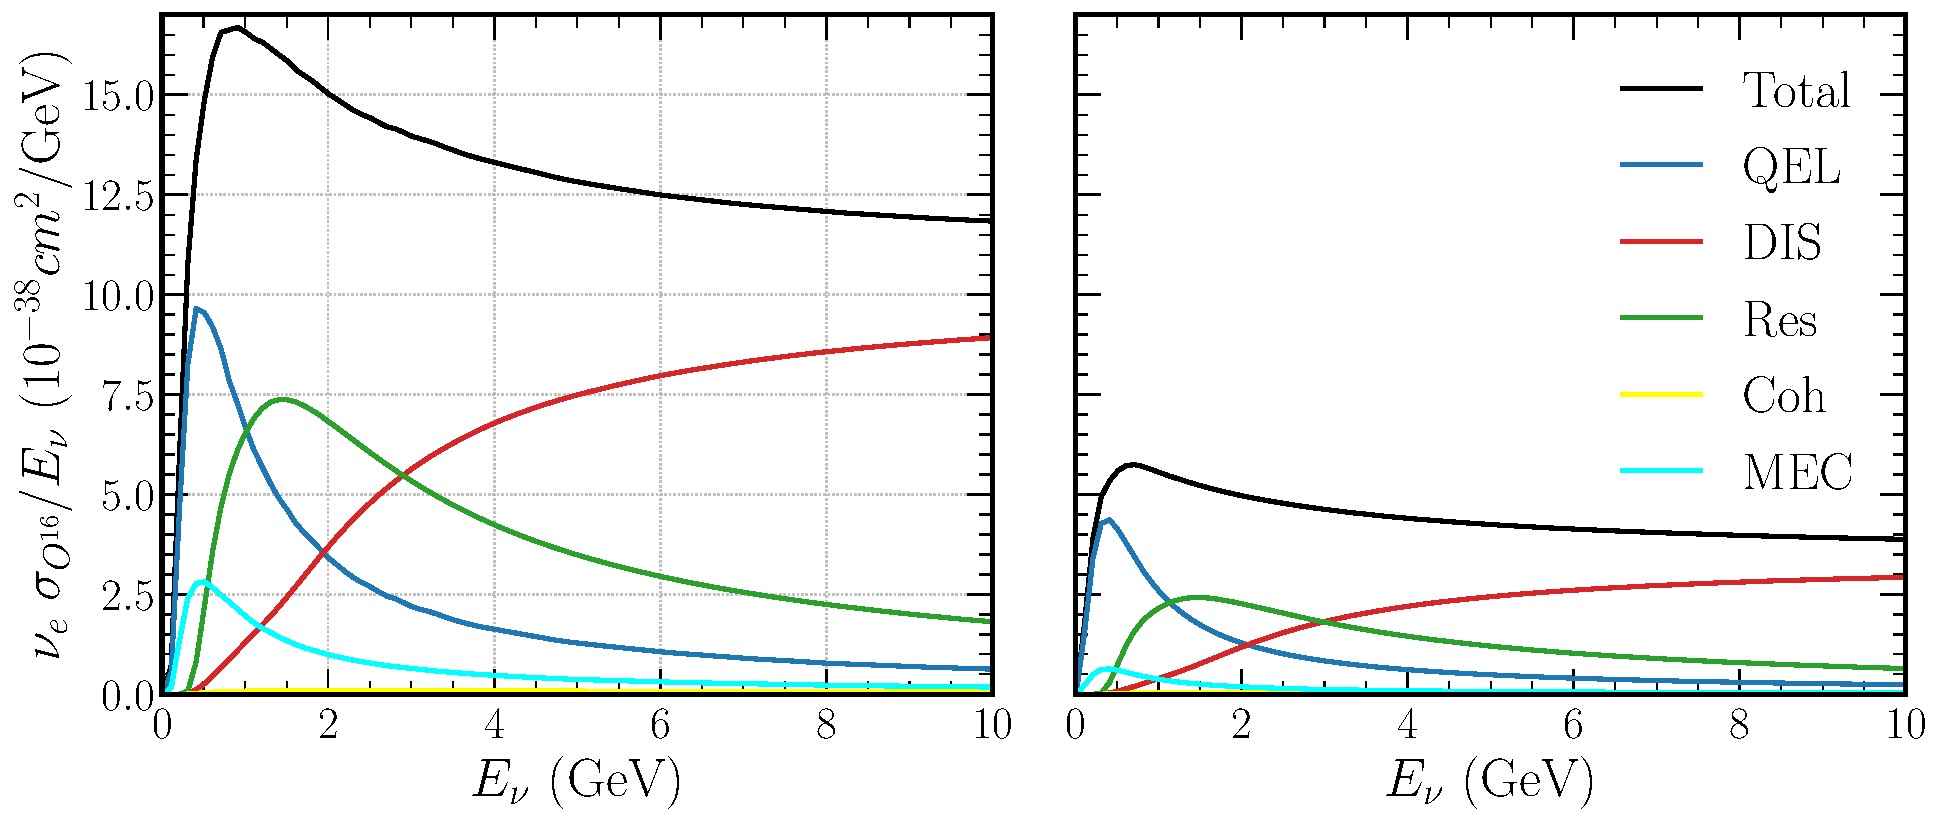
\includegraphics[width=\textwidth]{diagrams/3-theory/xsec_nu_e_O16.pdf}
    \caption[$\nu_{e}$ cross-sections on Oxygen-16]
    {Example \textsc{Genie} cross-sections divided by neutrino energy for CC $\nu_{e}$ (left) and
        NC $\nu_{e}$ (right). Shown are the total and contributing process cross-sections on
        Oxygen-16. Note how the total cross-section approaches a linear dependence on energy and
        the NC cross-sections are smaller than their CC counterparts. See
        Ref.~\cite{andreopoulos2015} for generation details.}
    \label{fig:xsec_nu_e_O16}
\end{figure}

\begin{figure} % TAU CROSS-SECTION DIAGRAM %
    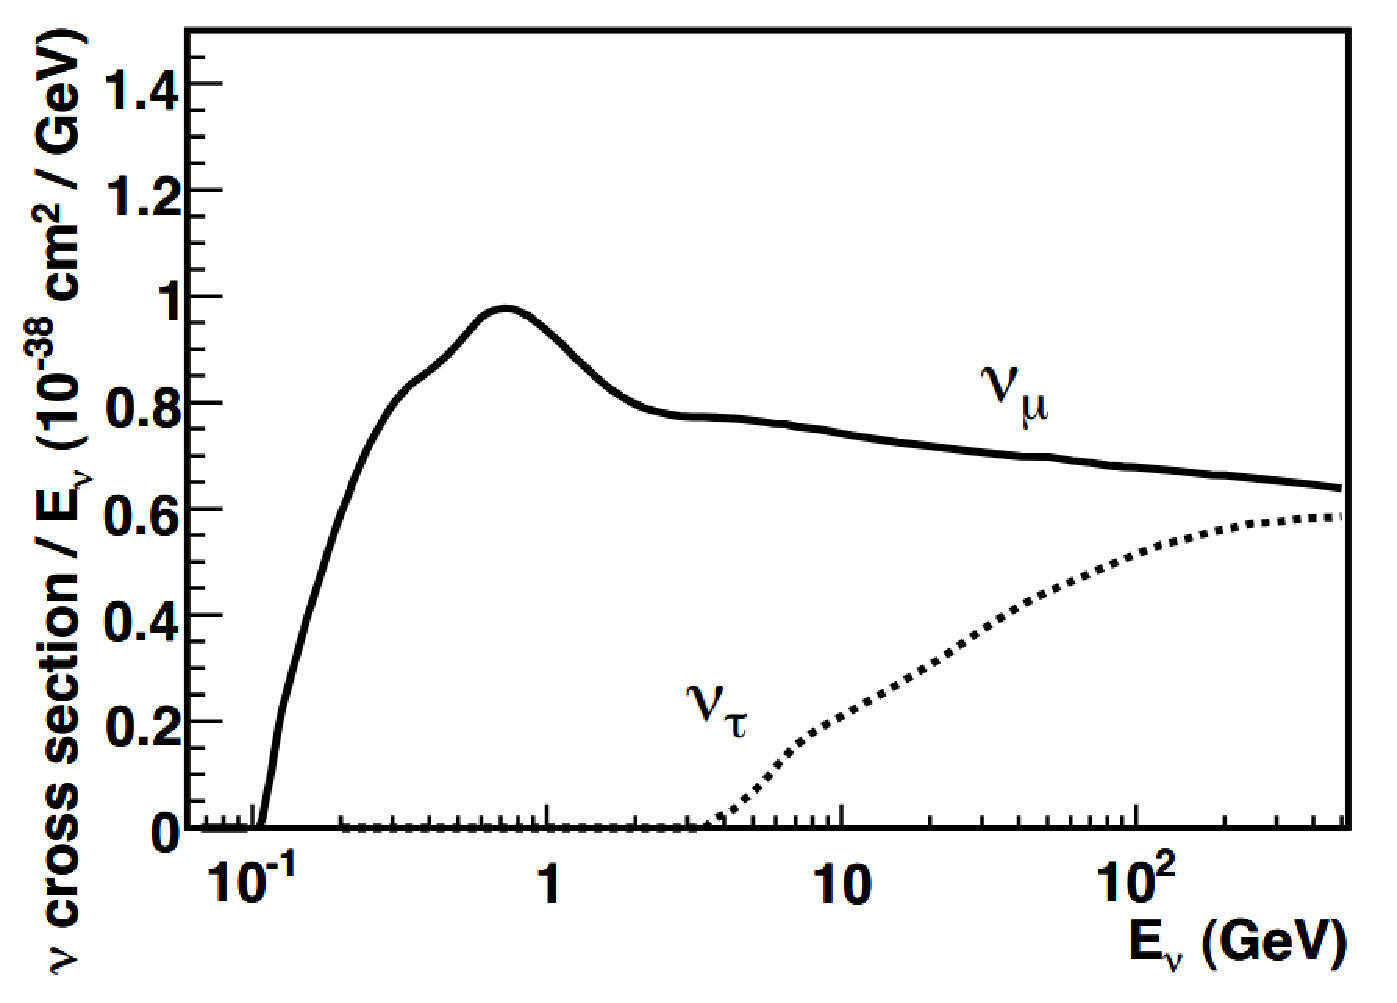
\includegraphics[origin=c,width=0.5\textwidth]{diagrams/3-theory/tau_comparison.pdf}
    \caption[Total charged-current cross-sections of $\nu_{\mu}$ and $\nu_{\tau}$]
    {Comparison of the total CC interaction cross-sections per nucleon divided by the neutrino
        energy for $\nu_{\mu}$ and $\nu_{\tau}$. Figure taken from Ref.~\cite{formaggio2012}.}
    \label{fig:tau_comparison}
\end{figure}

\section{Current status and the future} %%%%%%%%%%%%%%%%%%%%%%%%%%%%%%%%%%%%%%%%%%%%%%%%%%%%%%%%%%
\label{sec:theory_status} %%%%%%%%%%%%%%%%%%%%%%%%%%%%%%%%%%%%%%%%%%%%%%%%%%%%%%%%%%%%%%%%%%%%%%%%

The three-component representation of the PMNS matrix presented in Eq.~\ref{eq:matrix} splits our
understanding of neutrino oscillations into three sectors. Historically, the sectors corresponded
to experiments observing different sources of neutrinos, from either the Sun, atmosphere or
nuclear reactors. Hence the standard names given to each: the \emph{solar sector},
\emph{atmospheric sector}, and \emph{reactor sector}. However, it is perhaps more rigorous to
think of each sector as corresponding to the parameters they encompass: $\Delta m^{2}_{21}$ and
$\theta_{12}$ for solar, $\Delta m^{2}_{32}$ and $\theta_{23}$ for atmospheric, and $\theta_{13}$
for reactor.

During the last couple of decades, the focus of neutrino experiments across all sectors has
shifted from the discovery of neutrino fundamentals to the precise measurement of oscillation
parameters. This change has led to a corresponding shift into using increasingly abundant neutrino
sources (such as accelerator neutrino beams) and larger and larger detectors. Here we outline the
current status, open questions, and future for neutrino physics.

\subsection{Current status} %%%%%%%%%%%%%%%%%%%%%%%%%%%%%%%%%%%%%%%%%%%%%%%%%%%%%%%%%%%%%%%%%%%%%%
\label{sec:theory_status_current} %%%%%%%%%%%%%%%%%%%%%%%%%%%%%%%%%%%%%%%%%%%%%%%%%%%%%%%%%%%%%%%%

Global fits to neutrino oscillation data best summarise the current state of neutrino physics.
These aggregate the latest experimental results to constrain the neutrino oscillation parameters.
The best-fit results from one such fit, NuFIT~\cite{esteban2019, esteban2020}, are shown in
Fig.~\ref{fig:best_fit}. A detailed overview of other global fits is given in The Particle Data
Group's 2020 Review of Particle Physics~\cite{particle2020}. In summary, all mixing angles
$\theta_{12}$, $\theta_{23}$, and $\theta_{13}$ are found to be non-zero and $\Delta m^{2}_{21}$
is found to be much smaller than $\Delta m^{2}_{32}$.

\begin{figure} % BEST FIT DIAGRAM %
    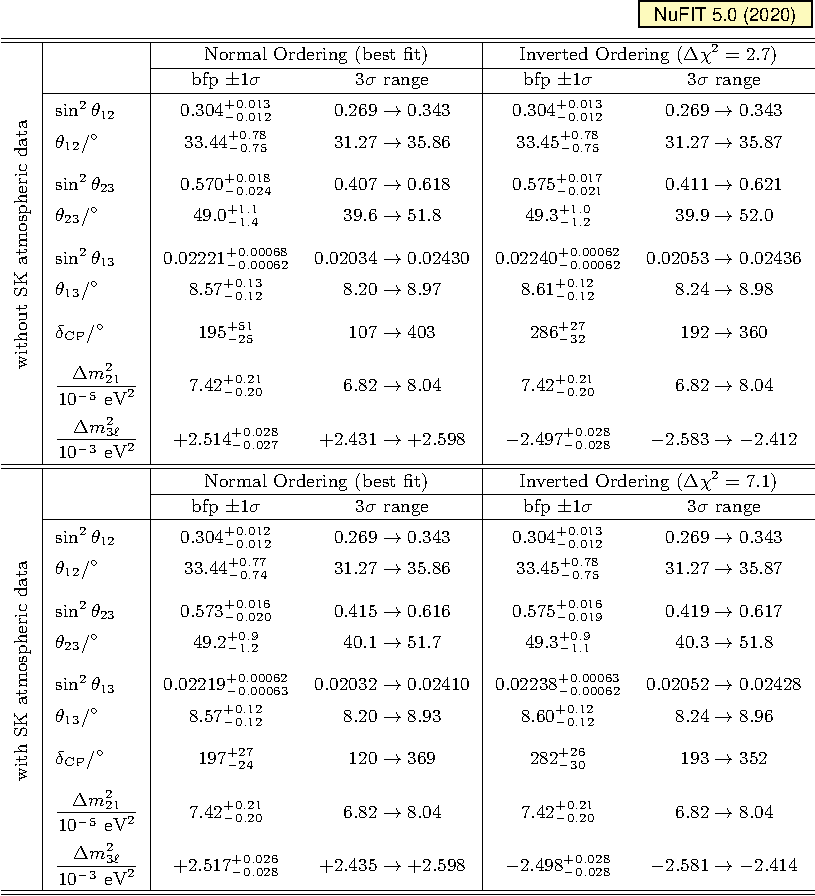
\includegraphics[origin=c,width=0.8\textwidth]{diagrams/3-theory/best_fit.pdf}
    \caption[Three-flavour results from the NuFIT v5.0 global neutrino oscillation fit]
    {Three-flavour results from the NuFIT v5.0 global fit as of July 2020, showing both 1$\sigma$
        uncertainties and $\pm 3 \sigma$ ranges. The first column shows results for an assumed
        normal hierarchy while the second for an inverted hierarchy. The lower section includes
        atmospheric neutrino data from the Super-Kamiokande experiment, while the upper section
        does not. Figure taken from Ref.~\cite{esteban2020}.}
    \label{fig:best_fit}
\end{figure}

\subsubsection*{Solar parameters: $\theta_{12}$ and $\Delta m^{2}_{21}$} %%%%%%%%%%%%%%%%%%%%%%%%%

Current best fit results for the solar sector parameters yield $\theta_{12}\sim34^{\circ}$ with
$\sim1.5^{\circ}$ of uncertainty, and $\Delta m^{2}_{21}\sim7.4\times10^{-5}\eV^{2}$ with
$\sim0.4\times10^{-5}\eV^{2}$ of uncertainty.

These results primarily come from a range of historical and currently running experiments studying
neutrinos generated by the Sun: the radiochemical chlorine-based Homestake~\cite{cleveland1998};
the gallium-based GALLEX~\cite{kaether2010} and SAGE~\cite{abdurashitov2009}; the deuterium
Cherenkov SNO~\cite{maneira2011}; the water Cherenkov Super-Kamiokande~\cite{hosaka2006,
    cravens2008, abe2011_super, nakano2017}; and the liquid scintillator detector
Borexino~\cite{bellini2011, bellini2010, bellini2014}. Most of which were mentioned previously in
Section.~\ref{sec:theory_history_osc}, originally involved in studying the solar neutrino problem.

Additionally, by locating a \unit{1}{\text{kton}} liquid scintillator detector between several
nuclear reactors, the KamLAND experiment has probed the solar sector in a terrestrial setting
using reactor antineutrinos~\cite{gando2011}. Unlike solar neutrinos, which are heavily influenced
by the high electron density of the Sun and the subsequent MSW effect, the antineutrinos detected
by KamLAND were not influenced, removing any measurement ambiguity.

\subsubsection*{Atmospheric parameters: $\theta_{23}$ and $\Delta m^{2}_{32}$} %%%%%%%%%%%%%%%%%%%

Current best fit results for the atmospheric sector parameters yield $\theta_{23}\sim48^{\circ}$
with $\sim2^{\circ}$ of uncertainty, and $\Delta m^{2}_{32}\sim2.45\times10^{-3}\eV^{2}$ (assuming
normal hierarchy as discussed in Section.~\ref{sec:theory_status_open}) with
$\sim0.03\times10^{-3}\eV^{2}$ of uncertainty. These results come from one of two primary sources.

Firstly, experiments studying atmospheric neutrinos generated in the upper atmosphere by cosmic
rays, such as IceCube~\cite{karle2003, aartsen2015} and the previously mentioned
Super-Kamiokande~\cite{abe2018}. IceCube is a neutrino observatory based at the Amundsen-Scott
South Pole Station in Antarctica, consisting of strings of PMTs embedded deep within the ice.
Whilst, Super-Kamiokande is a large \unit{50}{\text{kt}} water Cherenkov detector, equipped with
11000 PMTs, and located \unit{1}{\text{km}} underground in Gifu Prefecture, Japan.

Furthermore, \emph{long-baseline accelerator experiments} measuring
$P(\nu_{\mu}\rightarrow\nu_{\mu})$ from accelerator beam generated muon neutrinos over a
long-baseline of many hundreds of kilometres are sensitive to the atmospheric parameters. Such
experiments include: MINOS~\cite{adamson2013_1, adamson2013_2}(now complete) and
\nova~\cite{acero2019, himmel2020} using a beam generated at Fermilab with detectors in northern
Minnesota, and T2k~\cite{dunne2020} using a beam generated at J-PARC (on the east coast of Japan)
and using the Super-Kamiokande detector described above.

\subsubsection*{Reactor parameter: $\theta_{13}$} %%%%%%%%%%%%%%%%%%%%%%%%%%%%%%%%%%%%%%%%%%%%%%%%

The most recent parameter to be measured and found to be non-zero is $\theta_{13}$, with current
best fit results yielding a value of $\theta_{13}\sim8.5^{\circ}$ with $\sim0.25^{\circ}$ of
uncertainty (note that this is now the most tightly constrained of all the angles).

Primarily, $\theta_{13}$ measurements come from reactor experiments measuring electron
antineutrino disappearance, $P(\bar{\nu}_{e}\rightarrow\bar{\nu}_{e})$. The Daya Bay~\cite{an2012,
    an2017}, RENO~\cite{ahn2012, bak2018}, and Double Chooz~\cite{abe2012} experiments located in
China, South Korea, and France respectively all published the strongest results for this
measurement at a similar time.

Long-baseline accelerator experiments are also sensitive to $\theta_{13}$ through the electron
neutrino appearance channel $P(\nu_{\mu}\rightarrow\nu_{e})$. Measurements have been made by
MINOS~\cite{adamson2013_2}, T2k~\cite{abe2013}, and \nova~\cite{adamson2016_2} but with much
greater uncertainties than reactor experiments.

\subsection{Open questions} %%%%%%%%%%%%%%%%%%%%%%%%%%%%%%%%%%%%%%%%%%%%%%%%%%%%%%%%%%%%%%%%%%%%%%
\label{sec:theory_status_open} %%%%%%%%%%%%%%%%%%%%%%%%%%%%%%%%%%%%%%%%%%%%%%%%%%%%%%%%%%%%%%%%%%%

There are still many open questions (mainly ambiguities) regarding the parameters of the PMNS
matrix. \chips and other long-baseline accelerator experiments aim to help resolve those listed
here by studying the appearance of electron neutrinos in a muon neutrino beam. The approximate
oscillation probability for this transition including matter effects takes the
form~\cite{particle2020}:

\begin{align} % CHIPS PROB EQUATION %
    P(\nu_{\mu}\rightarrow\nu_{e},\bar{\nu}_{\mu}\rightarrow\bar{\nu}_{e})
     & \sim4\sin^{2}\theta_{13}\sin^{2}\theta_{23}\frac{\sin^{2}\Delta}{(1-A)^{2}} \nonumber     \\
     & + \alpha^{2}\sin^{2}2\theta_{12}\cos^{2}\theta_{23}\frac{sin^{2}A\Delta}{A^{2}} \nonumber \\
     & + 8\alpha J\cos(\Delta\pm\delta_{CP})\frac{\sin\Delta A}{A}\frac{\sin\Delta(1-A)}{(1-A)},
    \label{eq:chips_prob}
\end{align}

with

\begin{align} % CHIPS PROB PARTS EQUATION %
    J      & = \cos\theta_{12}\sin\theta_{12}\cos\theta_{23}
    \sin\theta_{23}\cos^{2}\theta_{13}\sin\theta_{13},       \\
    \Delta & = \frac{\Delta m^{2}_{31}L}{4E_{\nu}},          \\
    A      & = \pm\frac{2E_{\nu}V}{\Delta m^{2}_{31}},       \\
    \alpha & = \frac{\Delta m^{2}_{21}}{\Delta m^{2}_{31}},
    \label{eq:chips_prob_parts}
\end{align}

where $V$ is the effective matter potential in the Earth's crust, and $\pm$ is positive for
neutrinos and negative for antineutrinos.

\subsubsection*{Octant of $\theta_{23}$} %%%%%%%%%%%%%%%%%%%%%%%%%%%%%%%%%%%%%%%%%%%%%%%%%%%%%%%%%

The mixing angle $\theta_{23}$ is known to be non-zero and large. Initially thought to be maximal
such that $\theta_{23}=\pi/4=45^{\circ}$, it is now known that this is not the case. What it is
still unclear is if $\theta_{23}<45^{\circ}$ or $\theta_{23}>45^{\circ}$, commonly referred to as
the octant. Although easily measured be studying $\nu_{\mu}$ disappearance, a degeneracy in the
oscillation probability removes the ability to determine the octant. However, $\nu_{e}$ appearance
via the first term in Equation.~\ref{eq:chips_prob} allows for the octant to be resolved. Current
results suggest the $\theta_{23}>45^{\circ}$ octant is preferred; however, a significant
measurement is yet to be made.

\subsubsection*{Mass hierarchy} %%%%%%%%%%%%%%%%%%%%%%%%%%%%%%%%%%%%%%%%%%%%%%%%%%%%%%%%%%%%%%%%%%

The value of $\Delta m_{21}^2$ is known to be small and positive, meaning that $m_{2}>m_{1}$ where
$m_{1}$ is defined to be the dominant mass state of the electron neutrino. However, the sign of
$\Delta m_{32}^2$ is still currently unknown. This allows for two possible scenarios, either
$m_1<m_2<m_3$, known as \emph{normal hierarchy}, or $m_3<m_1<m_2$, known as \emph{inverted
    hierarchy}, as illustrated in Fig.~\ref{fig:hierarchy}. Resolving this ambiguity will
significantly improve the ability of experiments to both determine the value of $\delta_{CP}$
(discussed next) and discover if neutrinos are Dirac or Majorana in nature.

Oscillations in vacuum are not sensitive to the sign of the $\Delta m_{kj}^{2}$ parameters.
However, matter effects allow for the sign to be determined. Long-baseline $\nu_{e}$ appearance is
sensitive to the sign of $\Delta m_{32}^2$ via the $\Delta$, $A$, and $\alpha$ parameters in
Equation.~\ref{eq:chips_prob}. Furthermore, determining the hierarchy is also possible using
future reactor experiments such as JUNO~\cite{an2016}.

\begin{figure} % MASS HIERARCHY DIAGRAM %
    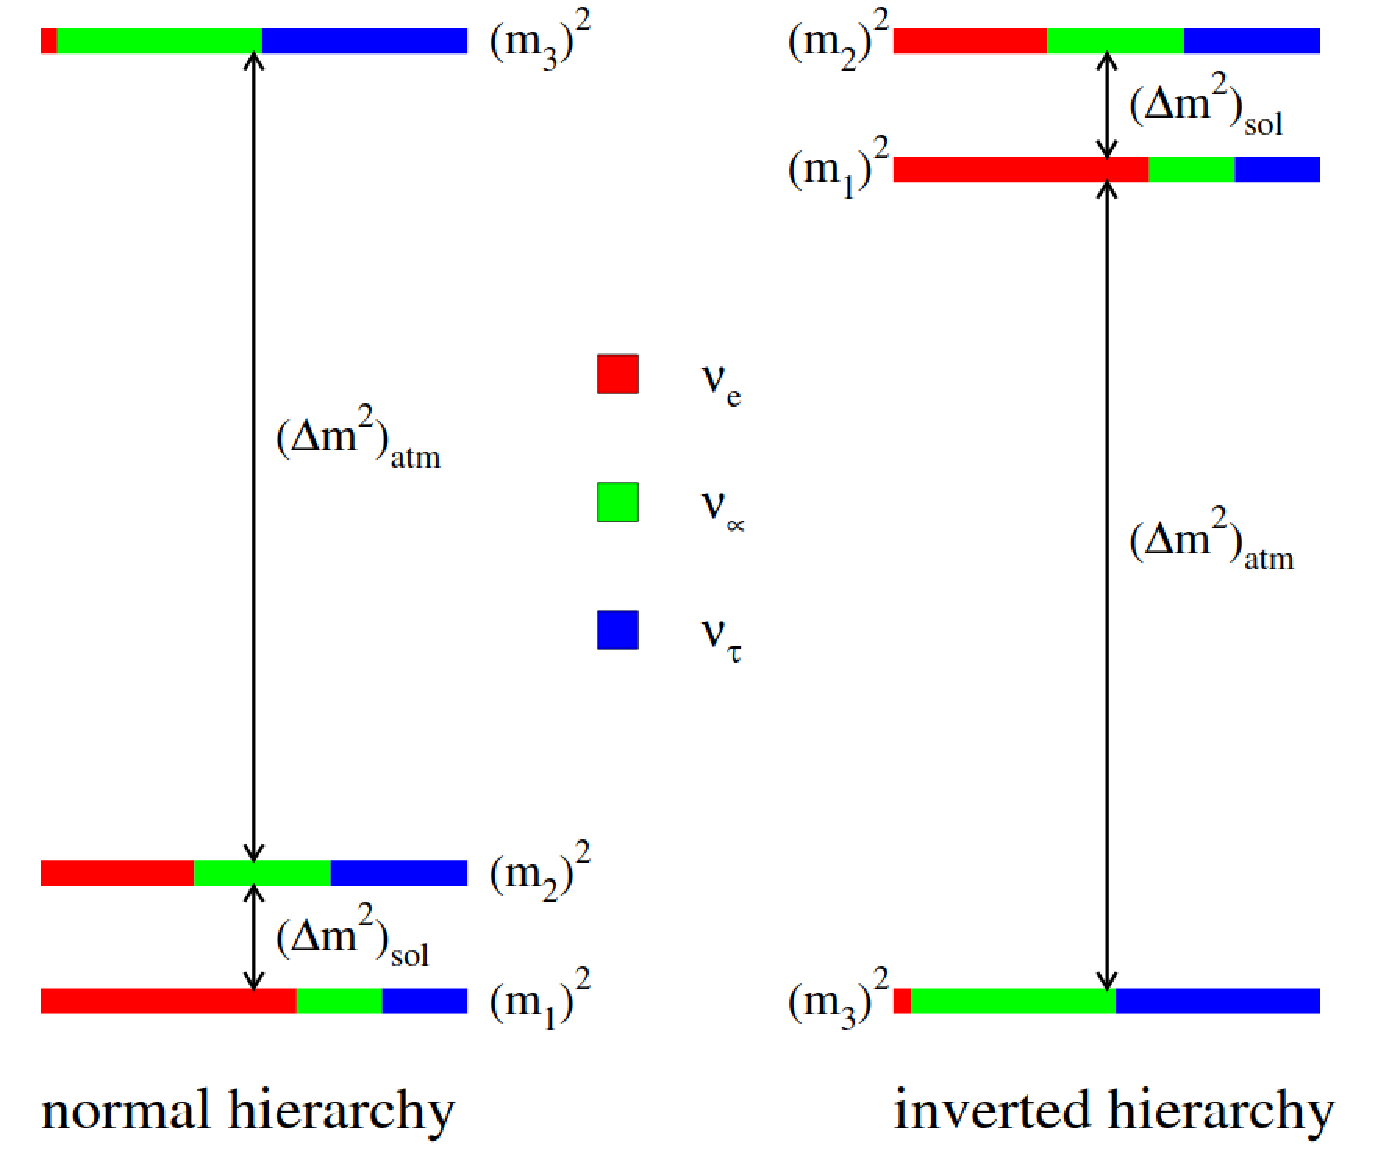
\includegraphics[origin=c,width=0.6\textwidth]{diagrams/3-theory/hierarchy.pdf}
    \caption[Illustration of the two neutrino mass hierarchies]
    {Illustrated diagram of the two neutrino mass hierarchies. The atmospheric (atm) and solar
        (sol) naming convention is used for the mass differences. The sign of $\Delta m_{21}^{2}$
        (sol) is small and positive, while the sign of $\Delta m_{32}^{2}$ (atm) is unknown.
        Figure taken from Ref.~\cite{gouvea2013}.}
    \label{fig:hierarchy}
\end{figure}

\subsubsection*{CP-violation} %%%%%%%%%%%%%%%%%%%%%%%%%%%%%%%%%%%%%%%%%%%%%%%%%%%%%%%%%%%%%%%%%%%%

The current level of CP violation observed in the quark sector does not fully explain the
matter-antimatter asymmetry of the universe. However, if CP violation is shown to exist in the
leptonic sector, leptogenesis models of the early universe allow this to go some way to resolving
the issue. Neutrino CP violation, when $P(\nu_{\alpha}\rightarrow\nu_{\beta}) \neq
    P(\bar{\nu}_{\alpha}\rightarrow\bar{\nu}_{\beta})$, is possible according to the PMNS matrix when
$\delta_{CP}$ is not 0 or $\pi$. $\nu_{e}$ appearance, sensitive to $\delta_{CP}$ via the third
term in Equation.~\ref{eq:chips_prob} is the most promising channel for measurement. The
oscillation probabilities are seen to change significantly with $\delta_{CP}$, as shown in
Fig.~\ref{fig:osc_cp_probs}. Current results from both \nova~\cite{acero2019} and
T2k~\cite{abe2018_2} hint at a possible non-zero value; however, a significant measurement is yet
to be made.

\begin{figure} % OSCILLATION CP PROBS DIAGRAM %
    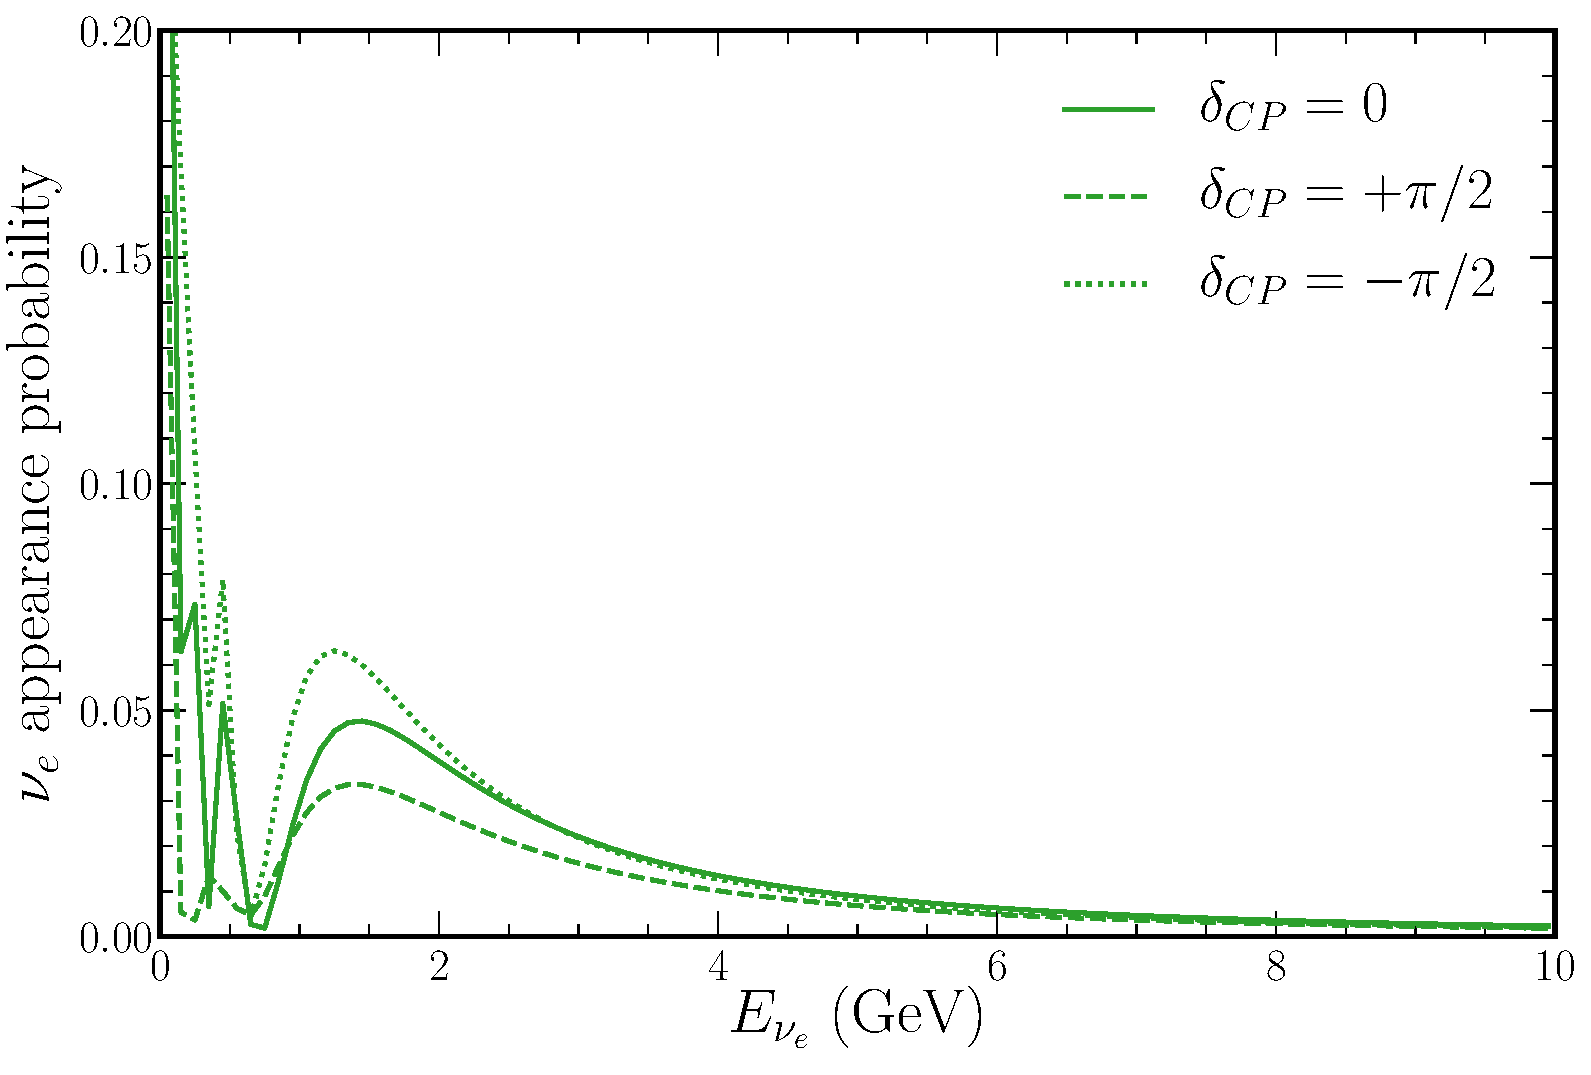
\includegraphics[origin=c,width=0.7\textwidth]{diagrams/7-results/explore_osc_cp_probs.pdf}
    \caption[$\nu_{e}$ appearance probability for different $\delta_{CP}$ values]
    {Appearance probability of $\nu_{e}$ oscillating from $\nu_{\mu}$ at $L=712$ km. The
        oscillations are show for three different values of $\delta_{CP}$.}
    \label{fig:osc_cp_probs}
\end{figure}

\subsection{The future} %%%%%%%%%%%%%%%%%%%%%%%%%%%%%%%%%%%%%%%%%%%%%%%%%%%%%%%%%%%%%%%%%%%%%%%%%%
\label{sec:theory_status_future} %%%%%%%%%%%%%%%%%%%%%%%%%%%%%%%%%%%%%%%%%%%%%%%%%%%%%%%%%%%%%%%%%

The current generation of long-baseline accelerator experiments (\nova and T2K) is not expected to
unambiguously determine the octant of $\theta_{23}$, the mass hierarchy, or the value of
$\delta_{CP}$. To finally determine the answers to these questions, primarily two next-generation
experiments are planned. The USA based Deep Underground Neutrino Experiment (DUNE) and
Hyper-Kamiokande in Japan. Both will have rich neutrino physics programs alongside their primary
goals, studying atmospheric and supernova neutrinos as well as nucleon decays.

DUNE~\cite{acciarri2016, abi2020}, will consist of four \unit{10}{\text{kt}} liquid argon time
projection chambers (LArTPCs) located \unit{1.5}{\text{km}} underground at the Sanford Underground
Research Facility, South Dakota. This location is the same as the Homestake mine chlorine
experiment previously mentioned in Section.~\ref{sec:theory_history_osc}. LArTPCs have been chosen
as they provide excellent track reconstruction and particle identification performance.

The DUNE experiment will also use a new high intensity beam constructed at Fermilab
(\unit{1285}{\text{km}} away) named the Long-Baseline Neutrino Facility (LBNF). Replacing the
current \unit{700}{\text{kW}} \numi (Neutrinos at the Main Injection) beam, LBNF is initially
planned to run at \unit{1.2}{\text{MW}}, but will eventually reach \unit{2.4}{\text{MW}}.

The initial cost estimate for DUNE combined with LBNF was forecast at between \$1.26 billion and
\$1.86 billion~\cite{dune_cost}. However, mainly due to rising underground excavation costs this
has recently risen to approximately \$2.6 billion~\cite{aip_budget}, an extremely high cost for a
neutrino experiment.

Hyper-Kamiokande~\cite{hyper_dr, hyperkamiok2014}, will be the next-generation replacement for the
currently running Super-Kamiokande detector. When completed, it will consist of two cylindrical
water Cherenkov detectors each \unit{60}{\text{m}} in height and \unit{74}{\text{m}} in diameter.
Both will be built under \unit{650}{\text{m}}  of rock at the Tochibora mine in Japan, close to
the current Super-Kamiokande location. New high-efficiency photomultiplier tubes will be used,
covering 40\% of the detector walls to record the Cherenkov radiation emitted from neutrino
events.

Moreover, there will be upgrades to the existing J-PARC neutrino beam, currently used by T2k. This
will increase the beam power from \unit{400}{\text{kW}} to \unit{1.3}{\text{MW}}. In total, the
Hyper-Kamiokande project is expected to cost approximately \$700 million.